\documentclass[12pt]{article}

\usepackage{tikz}


\begin{document}


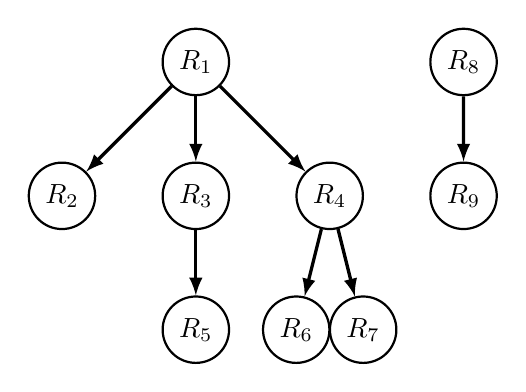
\begin{tikzpicture}[scale=0.85]
 \tikzstyle{quadri}=[circle,draw,text=black, thick]
 \tikzstyle{estun}=[->,>=latex,very thick]
 \node[quadri] (R1) at (0,3) {$R_1$};
 \node[quadri] (R2) at (-2,1) {$R_2$};
 \node[quadri] (R3) at (0,1) {$R_3$};
 \node[quadri] (R4) at (2,1) {$R_4$};
 \node[quadri] (R5) at (0,-1) {$R_5$};
 \node[quadri] (R6) at (1.5,-1) {$R_6$};
 \node[quadri] (R7) at (2.5,-1) {$R_7$};
 \node[quadri] (R8) at (4,3) {$R_8$};
 \node[quadri] (R9) at (4,1) {$R_9$};
 \draw[estun] (R1)--(R2);
 \draw[estun] (R1)--(R3);
 \draw[estun] (R1)--(R4);
 \draw[estun] (R3)--(R5);
 \draw[estun] (R4)--(R6);
 \draw[estun] (R4)--(R7);
 \draw[estun] (R8)--(R9);
\end{tikzpicture}



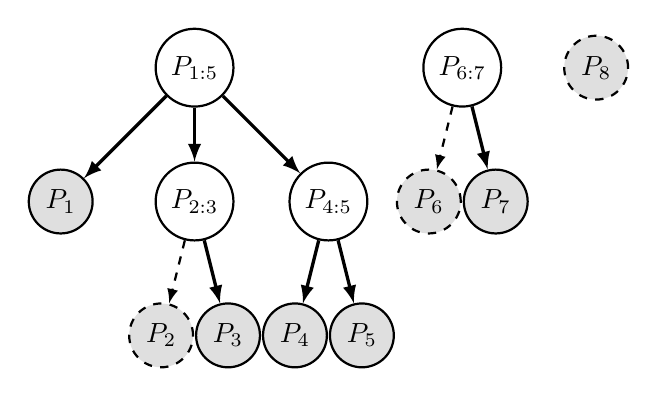
\begin{tikzpicture}[scale=0.85]
 \tikzstyle{quadri}=[circle,draw,text=black,thick]
 \tikzstyle{estun}=[->,>=latex,very thick]
 \node[quadri] (R1) at (0,3) {$P_{1:5}$};
 \node[quadri, fill=gray!25] (R2) at (-2,1) {$P_1$};
 \node[quadri] (R3) at (0,1) {$P_{2:3}$};
 \node[quadri] (R4) at (2,1) {$P_{4:5}$};
 \node[quadri, dashed,fill=gray!25] (P2) at (-0.5,-1) {$P_2$};
 \node[quadri,fill=gray!25] (R5) at (0.5,-1) {$P_3$};
 \node[quadri,fill=gray!25] (R6) at (1.5,-1) {$P_4$};
 \node[quadri,fill=gray!25] (R7) at (2.5,-1) {$P_5$};
 \node[quadri] (R8) at (4,3) {$P_{6:7}$};
 \node[quadri,dashed,fill=gray!25] (P6) at (3.5,1) {$P_6$};
 \node[quadri,fill=gray!25] (R9) at (4.5,1) {$P_7$};
 \node[quadri,dashed,fill=gray!25] (P8) at (6,3) {$P_8$};
 \draw[estun] (R1)--(R2);
 \draw[estun] (R1)--(R3);
 \draw[estun] (R1)--(R4);
 \draw[estun] (R3)--(R5);
 \draw[estun,dashed,thick] (R3)--(P2);
 \draw[estun] (R4)--(R6);
 \draw[estun] (R4)--(R7);
 \draw[estun] (R8)--(R9);
 \draw[estun,dashed,thick] (R8)--(P6);
\end{tikzpicture}






\end{document}
